\section{Auswertung}
\label{sec:Auswertung}

\begin{figure}
  \centering
  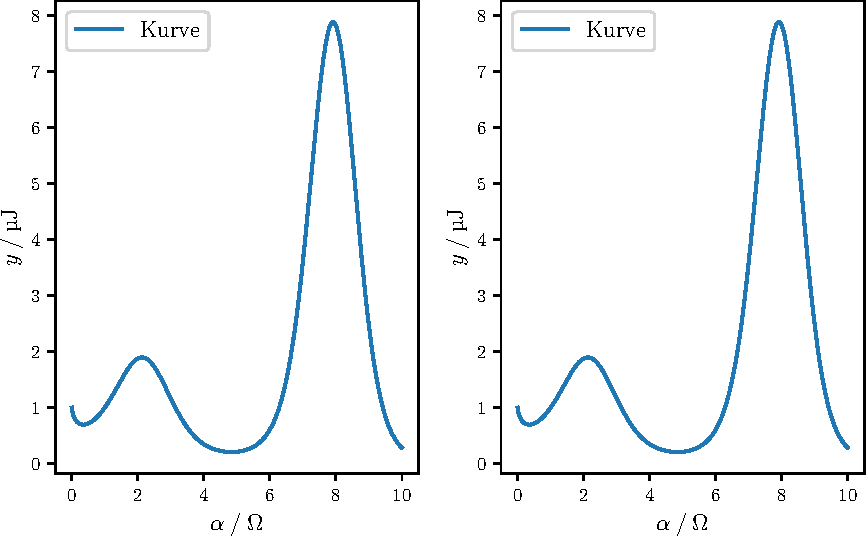
\includegraphics{plot.pdf}
  \caption{Plot.}
  \label{fig:plot}
\end{figure}

\begin{table}
  \centering
  \caption{Anzahl Maxima der Schwebung.}
  \label{tab:schwing_maxima}
  \begin{tabular}{c c}
      \toprule
      {$C_K \:/\: \si{\nano\farad}$} & Schwingungsmaxima \\
      \midrule
      9.99  & 13 \\ 
      8.00  & 11 \\ 
      6.47  & 10 \\ 
      5.02 & 8 \\ 
      4.00 & 7 \\
      3.00 & 6 \\
      2.03 & 4 \\ 
      \bottomrule
  \end{tabular}
\end{table}

\begin{table}
  \centering
  \caption{Gemessene Frequenzen in Abhängigkeit der Kopplungskapazität}
  \label{tab:frequenzen}
  \begin{tabular}{c c}
      \toprule
      {Frequenz $F\;/\; \si{\kilo\hertz}$} & {$C_K \:/\: \si{\nano\farad}$} \\
      \midrule
      30.74 & 9.99 \\
      31.39 & 8.00 \\
      31.57 & 6.47 \\
      31.82 & 5.02 \\
      32.11 & 4.00 \\
      32.60 & 3.00 \\
      33.41 & 2.03 \\
      35.90 & 1.01 \\
      \bottomrule
  \end{tabular}
\end{table}


\begin{table}
  \centering
  \caption{Ich weiß noch nicht genau, was wir gemacht haben} %Hier müssen noch die Messungen mit den Kästchen mulitpliziert werden
  \label{tab:aufgabeC}
  \begin{tabular}{c c c c c}
      \toprule
      {Maxima 1 $\;/ \si{\kilo\hertz}$} & {Maxima 2 $\;/ \si{\kilo\hertz}$} & {$V_1 \:/\: \si{50 \milli\volt}$} & {$V_2 \:/\: \si{50 \milli\volt}$} & {$C_K \:/\: \si{\nano\farad}$} \\
      \midrule
      2.1 & 2.7 & 1.2 & 2.2 & 9.99 \\
      2.2 & 2.8 & 1.1 & 2.2 & 8.00 \\
      2.2 & 2.8 & 1.1 & 2.2 & 6.47 \\
      2.1 & 3.0 & 1.0 & 2.2 & 5.02 \\
      2.2 & 3.2 & 1.0 & 2.1 & 4.00 \\
      2.2 & 3.4 & 1.0 & 2.1 & 3.00 \\
      2.2 & 4.0 & 1.0 & 2.0 & 2.03 \\
      2.2 & 4.2 & 1.1 & 1.9 & 1.01 \\
      \bottomrule
  \end{tabular}
\end{table}



%Siehe \autoref{fig:plot}! Ich weiß nicht, was das hier überhaupt sein soll. Das mach ein Siehe Abbildung ! in das Protokoll.
% Aber wofür ist das gut?
